\documentclass[11pt]{article}

\usepackage{amsmath, amssymb}
\usepackage{microtype}
\usepackage{parskip}
\usepackage[margin=1.1in]{geometry}
\usepackage{enumitem}
\usepackage{xcolor}
\usepackage{booktabs}
\usepackage{tikz}

\setlist[enumerate,1]{label=\arabic*.}
\setlist[enumerate,2]{label=\theenumi\arabic*.}

\begin{document}

These exercises are contributed by Dr. Geoff Wild who taught the course a few years back. Some instructors in the past have used these exercises. 

\begin{enumerate}
  \item \textbf{Some modelling basics}
    \begin{enumerate}
      \item Benjamin Franklin has been credited with first proposing the model, ``time is money.'' Is Franklin's model dimensionally homogeneous? Explain.
      \item If you double the diameter of a circle, then by what factor do you expect its area to increase?
      \item The model for the relationship between a bird's weight and its body length presented in the main text was built by assuming birds were cubes. How would the model change if we assume, instead, that birds are tetrahedrons? Explain. 
      \item The logarithm of the volume of a sphere is an affine linear function of the logarithm of its diameter. If we were to plot this relationship what would the slope and intercept of the resulting line be? 
      \item Heat generated by metabolism must be dissipated, and so it has been predicted that metabolic rate scales with surface area.  Keeping this in mind, propose a scaling model for the relationship between body weight and metabolic rate. Is the relationship isometric or allometric?  What would the relationship look like if plotted in log-log space?
      \item When prescribing a drug, why might it be important to know if the dose scales isometrically or allometrically with a patient's weight?	
      \item A team of palaeontologists has discovered two {\it Tyrannosaurus rex} footprints. The first measures 85 cm in length and the second measures 70 cm in length, suggesting they were made by different dinosaurs. Based on these footprints predict how much heavier the first dinosaur was. What caveats should accompany your predictions? Would you be confident using a comparison between a {\it T. rex} footprint and a {\it Diplodocus} footprint in the same way? Explain. 
      \item Verify directly that $p_t = \frac{2}{3}\left(-\frac{1}{2}\right)^t + \frac{1}{3}$ satisfies the recursive equation in Example 1. Do the same for $p_t=\frac{1}{3}$. Can you suggest why we call $p_t = \frac{1}{3}$ an {\it equilibrium} and why we don't do the same for $p_t  = \frac{2}{3}\left(-\frac{1}{2}\right)^t + \frac{1}{3}$?
      \item Is the recursive model in Example 1 dimensionally homogeneous? Explain.
      \item In the text, we proposed $u = \lambda^t\, a$ as a model for population growth. Is this a useful model? If so, why? If not, then suggest ways to improve the model.
      \item The {\it doubling time} of a population, denoted $t_d$, is the time it takes to double in size. Suppose the growth of a population can be described by $u_t = \frac{3}{2} u_{t-1}$, where $t$ is time in hours. What is the doubling time of the population? Does your answer make sense? Why?
      \item An infectious-disease epidemic begins when 32 cases are discovered on Feb 1. Experts are not sure how long these 32 cases have been in the area, but data collected on the number of new infections during the first few days of the epidemic gives them the following: 
        \begin{center}
          \begin{tabular}{c|r}
            Date & Number of new cases \\
            \midrule
            %Feb 1 & 32 \\
            Feb 2 & 35 \\
            Feb 3 & 78 \\
            Feb 4 & 154 
          \end{tabular}
        \end{center}
        If we assume that $u_t$, the {\it total} number of cases of the disease on day $t$, follows $u_t = \lambda^t \, a$ for the first few weeks of the epidemic, how many new cases do you predict will occur on Feb 10? How would your prediction change if you assumed $u_t = m \, t + b$? What are the public-health consequences of making a poor assumption about the increase in the number of infections over time? 
      \item Carbon-14 is a radioactive isotope of carbon that can be used to determine the age of archaeological artefacts of biological origin. The half-life of Carbon-14 is approximately $5\, 730$ years, meaning that the initial amount of C-14 contained by a sample is decreased by $50\%$ after $5\, 730$ years. Based on this information, propose a model for the relationship between the amount of C-14 present in a sample and time.  
      \item An initial investment of $1000$ dollars increases in value at a rate of $2\%$ per year. At the end of every year (after the interest is paid) the investor withdraws $50$ dollars. Devise a recursive model for the relationship between the value of the investment this year and its value last year. Then, turn the recursive model into an explicit one for the relationship between investment value and time. Will the investment ever be worthless? 
    \end{enumerate}

  \item Introduction to Differential Equations
    \begin{enumerate}
      \item Classify the following differential equations according to their order and decide whether they are linear or non-linear. If linear, then classify further as homogeneous or inhomogeneous.
        \begin{enumerate}
          \item $u'(t) = u(t)$
          \item $u''(t) = 1$
          \item $u'(t) = t\,u(t)$
          \item $u''(t) = u'(t) + \sin t$
          \item $y'(x) = \sin y(x)$
          \item $y'(x) = \sin x + y(x)$
          \item $x''' = e^{x'} + x$
          \item $v'' - 2\, v' + v = 0$
        \end{enumerate}
      \item Solve the following:
        \begin{enumerate}
          \item $u'(t) = t^2 - 1$ with $u(0) = 1$
          \item $u'(t) = t + 2$ with $u(0) = 2$ 
          \item $u'(t) = -t^3+t-1$ with $u(-1) = 2$
          \item $u'(t) = 0$ with $u(0) = 5$
          \item $y''(x) = 2$ with $y'(0) = 1$ and $y(0) = -1$
          \item $y''(x) = -y(x)$ with $y'(0) = 1$ and $y(0) = 0$
          \item $u''(t) = u'(t)$ with $u(0) = 1$ and $u'(0) =1$.
        \end{enumerate}
      \item A first-order differential equation is {\it separable} if it can be written as $u'(t) = g(u(t))\, h(t)$. Provided $g(u(t))$ is non-zero, we can solve a separable differential equation by ``separating the variables.'' In other words, we can solve by dividing by $g$ and integrating as described in Section 2.1. Solve the following differential equations by separating the variables.  
        \begin{enumerate}
          \item $y'(x) = -y(x) + 1$ with $y(0)=0$ 
          \item $u'(t) =  u(t) + 1$ 
          \item $y'(x) = -x\, y(x)$
          \item $y'(x) = x \, y(x) - x$
          \item $y'(x) = e^x\, y(x) + e^x$.
          \item Under what conditions can we view a first-order linear differential equation as separable?
          \item Use a computer to create sketches of the solutions to parts (a) to (e).
        \end{enumerate}
      \item Solve the following:
        \begin{enumerate}
          \item $u'(t) + \frac{1}{t+1}\, u(t) = t$ with $u(0)=1$
          \item $u'(t) + \frac{1}{t+1}\, u(t) = t$ with $u(-2) = 0$
          \item $y'(x) = -x\, y(x) + x$
          \item $y'(x) = e^x\, y(x) + e^x$
          \item $u'(t) - \frac{1}{t+1}\, u(t) = t$
          \item $u'(t) = \frac{1}{t(t-1)} - \frac{1}{t-1}\, u(t)$
          \item $u''(x) = u'(x) + 1$
        \end{enumerate}			 
      \item Write down a first-order linear differential equation for which the given function is a solution:
        \begin{enumerate}
          \item $u(t) = e^{2\, t}$
          \item $u(t) = e^{-t^2/2} + 1$
          \item $u(t) = \frac{t}{2} + \frac{2}{t}$
          \item $y(x) = \dfrac{\sin x - \cos x}{x}$ 
        \end{enumerate}
      \item A linear combination of the functions $u_1(t)$ and $u_2(t)$ is expressed as, $a\, u_1(t) + b\, u_2(t)$, where $a$ and $b$ are constants. Show that if $u_1(t)$ and $u_2(t)$  both satisfy the same $n$th-order linear homogeneous differential equation then any linear combination of these functions does as well.
      \item An affine linear combination of the functions $u_1(t)$ and $u_2(t)$ is expressed as, $a\, u_1(t) + (1-a)\, u_2(t)$, where $a$ is a constant. Show that if $u_1(t)$ and $u_2(t)$  both satisfy the same $n$th-order linear  differential equation (homogeneous or inhomogeneous) then any affine linear combination of these functions does as well. 
      \item Let $g$ be a continuous function. Show that $u(t) = \int\limits_a^t g( u(s) ) \, ds$, with $a$ constant, solves $u'(t) = g(u(t))$.
      \item Show that $u(t) = \frac{1}{v(t)} \big( u(a)\, v(a) + \int\limits_a^t v(s)\, q(s)\, ds\big)$ satisfies the general form of a linear, first-order differential equation.
      \item Consider $u'(t) = a\, u(t) + b$ for $a,b\neq 0$. Find an equilibrium solution to this differential equation. Show that a solution to the differential equation can be constructed by adding the equilibrium solution you found to the solution to $u'(t) = a\, u(t)$.
      \item We can solve the initial value problem, $u'(t) = u(t)$ with $u(0) = 1$ using a definite integral. We rewrite the differential equation as $u'(s) = u(s)$ where $s$ is a placeholder variable. Proceeding as before we find $\int\limits_0^t \frac{u'(s)}{u(s)}\, ds = \int\limits_0^t ds$. A change of variable leads to $\int\limits_{u(0)}^{u(t)} \frac{du}{u} = \int\limits_0^t ds$ which is easily solved as $u(t) = e^t$. Use this approach to solve $u'(t) = ( u(t) )^2$ with $u(1) = \frac{1}{2}$.
      \item Consider a well-stirred tank that initially contains 3 kg of NaCl dissolved in 30-L of water. At time $t=0$ a solution containing $250$ g per L of NaCl begins to  flow into the tank at rate 15 mL per s. 
        \begin{enumerate}
          \item Suppose at time $t=0$ the solution inside the tank begins to be drained at a rate of 15 mL per s. How much NaCl do you expect to find in the tank in the long-run?
          \item Propose a model for the relationship between the amount of NaCl in the tank and time. Does your model match your expectations from part (a)?
          \item Now suppose that at time $t=0$ the solution inside the tank is drained at a rate of 20 mL per s. Propose a revised model for the   for the relationship between the amount of NaCl in the tank and time. At what point in time do your model's predictions break down? 
        \end{enumerate}
      \item A {\it Bernoulli equation} is a non-linear differential equation of the form $y'(x) + P(x)\, y(x) = Q(x) \, (y(x))^n$. An example of such an equation is the logistic model. Show that the {\it Bernoulli substitution} $u = y^{1-n}$ transforms a Bernoulli equation into one that is linear and of first order. Solve the following using a Bernoulli substitution
        \begin{enumerate}
          \item $x'(t) = \frac{1}{t} x(t) - t x(t)^4$ with $x(-1) = 1/2$
          \item $u''(x) = u'(x) \, ( \, 1 - u'(x) \,)$
        \end{enumerate}
      \item Redo Example 4 by modelling per-capita mortality as $r(N/K)^2$ and $r(N/K)^{1/2}$, respectively. What biological assumptions are we making about mortality in each case? What is the predicted relationship between population size and time in each case?
      \item Consider a species that occupies a large number of islands. The distribution of the species across all islands is maintained by a balance between local extinctions and colonizations. Devise a model for the relationship between the fraction of islands occupied by the species and time. Be clear to outline the assumptions you make, and be sure to describe your key predictions.
    \end{enumerate}

  \item Inexact Approaches to differential equations
    \begin{enumerate}
      \item Which of the following first-order differential equations are autonomous and which are not?

        \begin{minipage}{2in}
          \begin{enumerate}
            \item $u'(t) + u(t) = 1$
            \item $u'(t) + tu(t) = 0$
            \item $u'(t) - u(t) = \sin t$
            \item $y'(x) = y(x)^2$
          \end{enumerate}
        \end{minipage}
        \hspace{0.25in}
        \begin{minipage}{2.5in}
          \begin{enumerate}
            \item[(e)] $y'(x) = x^2y(x)$
            \item[(f)] $u' = (u+1)(u-1)$
            \item[(g)] $u'(t) = (u+t)(u-t)$
            \item[(h)] $y' = y(a - y)$, $a$ constant
          \end{enumerate}
        \end{minipage}
      \item Use a phase-line sketch to find equilibria of $u'=u^2-3u-4$ and classify the stability of each. Compare your approach to the one presented in Example 2.
      \item Find the equilibrium solutions to $u' = -(u^2-3u-4)$ and use a derivative condition to classify them according to their local stability.
      \item Write down an autonomous differential equation that has exactly two negative equilibria and exactly two positive equilibria. Ensure that equilibria, beginning with the smallest (i.e. most negative), alternate between asymptotically stable and unstable.
      \item Provide an example of an autonomous differential equation, $u' = g(u)$ with an asymptotically stable equilibrium $\bar u$ such that $g'(\bar u)$ is not negative.
      \item Provide an example of an autonomous differential equation, $u' = g(u)$ with an unstable equilibrium $\bar u$ such that $g'(\bar u)$ is not positive. 
      \item What do Exercises 5 and 6 tell you about the use of derivatives when assessing the stability of an equilibrium?
      \item Suppose that, if left unharvested, a fish stock grows according to $N'(t) = r \, N(t)\, (1 -N(t)/K)$, where $N(t)$ denotes the size of the stock (number of individuals) at time $t$. Suppose further that, when it is allowed, harvesting effectively imposes an additional per-capita mortality rate of $h$. 
        \begin{itemize}
          \item[(a)] Propose a recursive differential-equation model for the size of the harvested stock. What predictions does this model make?
          \item[(b)] Use the model you developed in (a) to state a new model that describes the relationship between the size of the stock and time. Use this model to confirm the predictions identified in (a).
          \item[(c)] If you were managing the stock you might recommend harvesting occur at the highest rate that also ensures sustainability. Based on the model you developed in (a), what is that rate? 
        \end{itemize}

      \item The solution to the initial value problem $u'(t) = \frac{t+1}{t-1} e^{-u(t)}$ with $u(\frac{3}{2}) = 0$ is 
        \[
          u(t) = \ln \bigg( t-\frac{1}{2} + 2\ln (2t-2)\bigg)
        \]
        which is a function whose graph is concave down. Would Euler's method overestimate or underestimate this exact solution? Explain. Verify your answer by using Euler's method to solve the problem on $(\frac{3}{2}, \frac{9}{2}]$ with $S=16$ subintervals (use a computer).
      \item 	Consider an enzyme that catalyzes the conversion of some substrate into a product. Let $u(t)$ be the fraction of the initial amount of substrate that remains in solution $t$ seconds following the addition of the enzyme. Then 
        \begin{equation}\label{eq:ivp}
          u'(t) = -\frac{V \, u(t)}{K + u(t)}, \quad u(0) = 1
        \end{equation}
        where $V$ is the rate at which the reaction proceeds when substrate is plentiful, and $K \ll 1$ is the {\it Michaelis constant} which is related to the availability of free enzyme in solution. It can be shown that $u(t)$ satisfies
        \begin{equation}\label{eq:soln}
          K \ln u(t) + u(t) = -V\, t + 1.
        \end{equation}
        Set $K=0.1$ and $V=2$ and solve the initial value problem in \eqref{eq:ivp} on $(0,1]$ using Euler's method with $S=4$. What challenges do you encounter? What can you do to overcome those challenges? Implement your strategy and develop a revised answer. Compare your revised answer to the exact solution in equation \eqref{eq:soln} using a plot.  
    \end{enumerate}

  \item Introduction to probability
    \begin{enumerate}
      \item Consider the experiment in which a coin is tossed exactly once. What is the sample space $\Omega$ for this experiment? List all events associated with the experiment.
      \item In Season 2 of the classic TV program {\it Corner Gas} (Episode 8: {\it Security Cam}), affable police officers Karen Pelly and Davis Quinton are asked about the odds of a riot breaking out in their local town, Dog River. The officers reply that the odds are 50:50, because a riot either breaks out or it doesn't. Do you agree with Karen and Davis? Why?
      \item One playing card is drawn from a standard, well-shuffled deck of $52$. What is the probability that the card is the Queen of Hearts? What is the probability that the card is a Queen or a Heart?
      \item If a pair of fair dice is rolled, then what is the probability that the sum of the numbers on the their faces is $12$? What is the probability that the sum is $7$? 
      \item A pair of fair dice is rolled, then the absolute value of the difference between the numbers shown on their faces, call it $D$, is determined. What is the most likely value of $D$?
      \item A fair die is rolled four times in succession. What is the probability that at least one of the numbers rolled is even?
      \item The {\it sensitivity} of the nasal-swab test for COVID-19 refers to the rate at which it correctly detects those who are infected by COVID-19. Express the sensitivity in terms of the probability of committing a type-II error.
      \item Estimate the sensitivity of the serum screen discussed in Example \ref{eg:triple}.
      \item Does increasing the sensitivity of a test necessarily decrease its specificity? Explain.
      \item (Due to Maynard Smith \cite{jms}) A woman of blood group O (genotype $OO$) gives birth to twins fathered by an $AB$ man (genotype $AB$). Given that the twins both belong to blood group $B$ (genotype $OB$) what is the probability they are monozygotic? {\it Hint:} use the observation that about 32\% of all twins are of opposite sex.
      \item Five friends -- Albert, Beatrice, Charles, Daphne, and Edward -- are doing a ``Secret Santa'' gift exchange. Each friend places their name into a hat and then each one draws one name at random from the hat. Each friend will secretly buy a gift for the person whose name they have drawn. What is the probability that no one gets their own name?
    \end{enumerate}

  \item Random variables and their applications

    \begin{enumerate}
      \item Given the following cumulative distribution function, sketch the corresponding probability mass function, or probability density function.
        \begin{center}
          \begin{tikzpicture}
            \node at (-2,2.5) {(a)};
            \draw[-latex] (-2,0)--(3,0) node[above] {$x$};
            \node at (-1,0) {$\circ$};
            \node at (-1,0.5) {$\bullet$};
            \draw (-1,0.5)--(-0.3,0.5);
            \node at (-0.25,0.5) {$\circ$};
            \node at (-0.25,1.5) {$\bullet$};
            \draw (-0.25,1.5)--(0.45,1.5);
            \node at (0.5,1.5) {$\circ$};
            \node at (0.5,2) {$\bullet$};
            \draw (0.5,2) -- (1.2,2);
            \node at (1.25,2) {$\circ$};
            \node at (1.25,2.25) {$\bullet$};
            \draw (1.25,2.25)--(2.75,2.25);
            %\node at (2,2.25) {$\circ$};
          \end{tikzpicture} 

          \begin{tikzpicture}
            \node at (-2,2.5) {(b)};
            \draw[-latex] (-2,0)--(3,0) node[above] {$x$};
            \draw (-1.5,0)--(-0.5,1)--(0.5,1)--(2,1.75)--(2.75,1.75);
          \end{tikzpicture}
        \end{center}
      \item Given the following probability mass function, or probability density function, sketch the corresponding cumulative density function.	
        \begin{center}
          \begin{tikzpicture}
            \node at (-2,2.5) {(a)};
            \draw[-latex] (-2,0)--(3,0) node[above] {$x$};
            \node at (-1,0) {$\circ$};
            \node at (-1,1.5) {$\bullet$};
            \node at (-0.25,0) {$\circ$};
            \node at (-0.25,0.75) {$\bullet$};
            \node at (0.5,0) {$\circ$};
            \node at (0.5,0.6) {$\bullet$};
            \node at (1.25,0) {$\circ$};
            \node at (1.25,0.75) {$\bullet$};
            \node at (2,0) {$\circ$};
            \node at (2,1.5) {$\bullet$};
          \end{tikzpicture} 

          \begin{tikzpicture}[yscale=5]
            \node at (-2,0.5) {(b)};
            \draw[-latex] (-2,0)--(3,0) node[above] {$x$};
            \draw[domain=-1.5:2.7,samples=100] 
            plot({\x}, {0.5*exp(-0.5*(\x+1.5))-0.025});
            \node at (-1.5,0) {$\circ$};
            \node at (-1.5,0.488) {$\bullet$};
          \end{tikzpicture}
        \end{center}
      \item Let $X$ be a continuous random variable with probability density function given in Figure \ref{fig:pdf}. What is the probability (a) that $X$ is between $-3/10$ and $1/5$? (b) that $|X|$ is greater than $1/4$? 
      \item A {\it binomial random variable} gives the number of success that result from a fixed number of independent experimental trials. The probability mass function for a binomial random variable is given by
        \[
          p(k)
          =
          \begin{cases}
            \dfrac{n!}{(n-k)!\, k!} s^k (1-s)^{n-k}
                        & 0 \leq k \leq n \\
            0 & \text{otherwise}
          \end{cases}
        \]
        where the positive integer $n$ represents the number of trials, and the real number $0<s<1$ gives the probability of success in any given trial. The exclamation mark represents the factorial function introduced back in Chapter 1.
        \begin{enumerate}
          \item Plot the cumulative distribution function for a binomial random variable with $n=3$ and $s=\frac{1}{4}$.
          \item If $X$ is a random variable that comes from a binomial distribution with $n=4$ and $s=\frac{1}{4}$ what is the probability that $X$ is even?
          \item Given that $X$ follows the distribution in part (a), detail a method for generating values of $X$ on a computer.
          \item Calculate the expectation and the variance of a random variable that follows a binomial distribution with $n=4$ and unspecified $s$.
        \end{enumerate}
      \item Let $X$ be a continuous random variable with probability density function $f(x)$ equal to $k\,x^2$ for $x$ between $1$ and $4$, and equal to zero elsewhere. 
        \begin{enumerate}
          \item Find the appropriate value of $k$, and generate fifty independent values of $X$ using a computer.
          \item Determine the expectation and the variance of $X$. Verify your answers using the numbers generated in part (a).
        \end{enumerate}
      \item Expectation is linear, which means that given two random variables $X$ and $Y$ and two constants $a$ and $b$, $E(aX+bY) = a\, E(X) + b\, E(Y)$. Use this idea to show that $\text{Var}(X)$ can be calculated as $E(X^2) - (E(X))^2$.
      \item Given that $a$ is a constant, show that $\text{Var} (a\, X) = a^2\, \text{Var}(X)$ and $\text{Var}(a + X) = \text{Var}(X)$.
      \item Consider a continuous random variable $X$ whose probability density function is given by $f(x) = 2 x$ for $0\leq x \leq 1$ (zero elsewhere). Plot the probability density function, find expectation of $X$ and the variance of $X$, and mark the expectation on the plot you create. Does $E(X)$ correspond to the highest point on the graph of $f(x)$? Is $E(X)$ found at the midpoint of the domain?
      \item Let $T$ denote the time it takes for an individual to recover from a particular infectious disease. We often model $T$ as an {\it exponential} random variable, with cumulative density function $F(t) = 1 - e^{-\gamma t}$ for $t\geq 0$. We commonly refer to $\gamma$ as the {\it recovery rate}, and measure it as inverse days. Use pairs of pseudorandom numbers to estimate the expected duration of an infection when the recovery rate is $\gamma = 3$ day$^{-1}$. 
      \item We can convert a continuous random variable $U$ that comes from a uniform distribution on $[0,1]$ into one with distribution function $F$ by determining $F^{-1}(U)$. Verify your answer to the previous problem by generating pseudorandom variables taken from an exponential distribution with $\gamma = 3$.    
      \item A geometric series is an infinite sum of the form
        \[
          \sum_{k=1}^\infty a\, r^{k-1} = a + a\, r + a\, r^2 + a\, r^3 + \ldots
        \]
        where $a$ and $r$ are constants. When $|r|<1$ it can be shown that
        \[
          \sum_{k=1}^\infty a\, r^{k-1} = \frac{a}{1-r}.
        \]	
        A {\it geometric random variable} can be used to model, among other things, the lifespan of an individual. If $s$ is the probability that an individual survives from one year to the next, then the probability that it dies in its $k$th year, where $k\geq 1$, is $p(k) = (1-s) s^{k-1}$. If we adopt such a model, then what is an individual's expected lifespan? {\it Hint:} what happens when you differentiate $s^k$ with respect to $s$? 
      \item Keno is a casino game in which players place bets on numbers from 1 to 80. Twenty numbers are then drawn randomly, and players receive payouts based on, among other things, the number of correct bets they made. What are the potential risks faced by a casino that automates its keno game using a random number generator\footnote{In 1994, the Montreal Casino lost 600 000 CAD when a keno player was able to correctly wager on 19 of the 20 numbers drawn three times in a row. The numbers in the keno game had been chosen by a random number generator.}?
      \item The average grade on last year's biology final was $72$ with a {\it standard deviation} of $\sqrt{s^2} = 7$. The average grade on last year's calculus final was $61$ with a standard deviation of $\sqrt{s^2}=4$. Lisa scored a $75$ on the biology final and a $71$ on the calculus final. Compare Lisa's relative performance in biology and calculus ({\it Hint:} how many standard deviations from the mean was Lisa in each exam?). What relevance does this kind of relative comparison have for the discussion in Example \ref{eg:ttest}?
      \item (Due to Zar \cite{zar}) A species of marine arthropod lives in water than contains 32 mmol of calcium per kg. Biologists collected a number of specimens and measured the calcium concentration in the fluid found inside their body cavity, also known as the {\it coelom}. Based on the data below, can we conclude that the concentration of calcium in the coelomic fluid of this arthropod is less than that of its environment? Explain by making reference to the probability of committing a type-I error.

        \begin{center}
          \begin{tabular}{cc}
            \hline
            Specimen \# 
                        & [ Ca ] (mmol/kg fluid) \\
                        \hline
            1 & 28 \\
            2 & 27 \\
            3 & 29 \\
            4 & 29 \\
            5 & 30 \\
            6 & 30 \\
            7 & 31 \\
            8 & 30 \\
            9 & 33 \\
            10 & 27 \\
            11 & 30 \\
            12 & 32 \\
            13 & 31 \\
            \hline
          \end{tabular}
        \end{center}	 
    \end{enumerate}

  \item Vectors and Functions of vectors
    \begin{enumerate}
      \item Show that $(c \vec{x}) \bullet \vec{y}=c(\vec{x}\bullet \vec{y})$ for any constant $c$.
      \item Express $\vec{u}={-1\brack -1}$ as a linear combination of $\vec{x}_1 = {1\brack 2}$ and $\vec{x}_2 = {-1\brack 3}$. That is, find the constants $c_1$ and $c_2$ such that $\vec{u} = c_1\, \vec{x}_1+ c_2\, \vec{x}_2$.	
      \item Can ${3\brack 1}$ be expressed as a linear combination of ${1 \brack 1}$ and ${2\brack 2}$? Explain.
      \item Show that $\vec{a} \bullet (c_1\, \vec{x} + c_2\, \vec{y})=c_1 \vec{a}\bullet \vec{x} + c_2 \, \vec{a}\bullet \vec{x}$, where $\vec{a}$, $\vec{x}$, and $\vec{y}$ are all vectors with $n$ elements, and where $c_1$ and $c_2$ are constants. What does the equality tell you about the effect a linear function has on linear combinations of its arguments?
      \item Explain why the real-valued function $f(x_1, x_2) = x_1^2 + x_2^2$ is not linear.
      \item Find the area of the parallelogram spanned by the vectors $\vec{x}_1$ and $\vec{x}_2$ in Exercise 3.
      \item Let $\vec{F}(\vec{x}) = {1 \ 1 \brack 1 \ 2}\vec{x}$.
        (a) Find $\vec{F}({-1\brack 1})$. (b) Sketch the vector field $\vec{F}$ in the style of Figure \ref{fig:vf}. What kind of movement does your plot suggest? (c) Sketch the image of the unit square in the range of $\vec{F}$. Is $\vec{F}$ invertible? Why?
      \item Consider the following matrix-vector pair:
        \[
          A = 
          \begin{bmatrix}
            1 & 2 & 3 \\ 4 & 5 & 6			
          \end{bmatrix}
          \quad
          \vec{x}
          =
          \begin{bmatrix}
            1 \\ 2
          \end{bmatrix}.
        \]
        Can you compute $A\, \vec{x}$? If so, then what is it? If not, then why?
      \item Give two examples of a two-dimensional square matrix that is not invertible.
      \item Determine whether each of the following defines an invertible vector field.
        \[
          \text{(a)}
          \quad
          \begin{bmatrix}
            -1 & 0 & 2 \\ 
            1 & 1 & 1 \\ 
            2 & -1 & 1
          \end{bmatrix}
          \quad 
          \text{(b)}
          \quad
          \begin{bmatrix}
            1 & 0 & 1\\ 
            -1& 2 & 1\\
            0 & 2 & 2
          \end{bmatrix}
          \quad
          \text{(c)}
          \quad
          \begin{bmatrix}
            0 & -2 & 1 \\
            1 & 0 & 1 \\
            0 & 0 & -1
          \end{bmatrix}
        \]
      \item  Let $A = {1 \quad 2\brack 2\ \, -1}$ and $B={0\, \ -1 \brack 2 \quad 1}$. Define $\vec{F}(\vec{x}) = A\, \vec{x}$ and $\vec{G}(\vec{x}) = B\, \vec{x}$. Find the matrix associated with $\vec{F} \circ \vec{G}$ and $\vec{G} \circ \vec{F}$.
      \item Consider the matrix
        \[
          A =
          \begin{bmatrix}
            2 & 1 & 1 \\ -1 & -1 & 1 \\ 1 & 0 & 2
          \end{bmatrix}.
        \]
        verify that $A$ is not invertible and find a non-zero vector $\vec{x}$ such that $A\, \vec{x}$ is equal to the zero vector.
      \item (a) Develop a biological scenario that is consistent with the information provided in the network below. (b) Devise a vector field that can be used to model the dynamics of the population. (c) Use your vector field to determine the distribution of individuals in the population after three years, assuming that there were initially two individuals in each category. 
        \begin{center}
          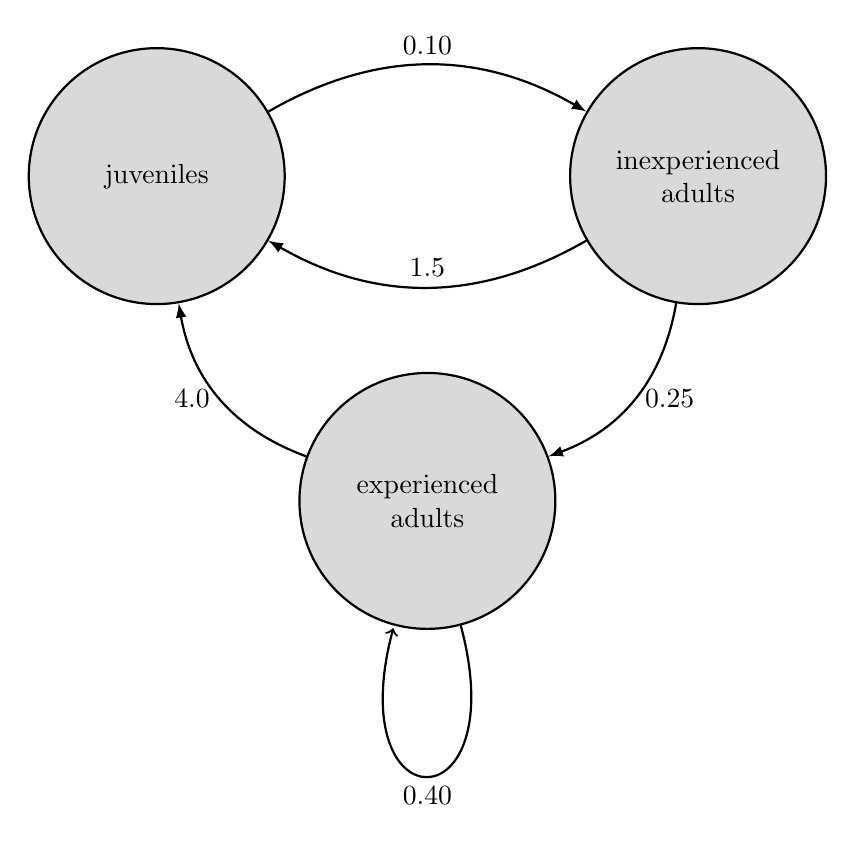
\begin{tikzpicture}[thick, class/.style={circle,draw,minimum size=3.25cm,fill=gray!30,align=center},scale=2.75]
            \node[class] (A) at ( 1.25,1.25) {inexperienced\\ adults};
            \node[class] (J) at (-1.25,1.25) {juveniles};
            \node[class] (A2) at (0,-0.25) {experienced\\ adults};
            %
            \path[-latex] (J) edge [bend left] node[above] {$0.10$} (A);
            \path[-latex] (A) edge [bend left] node[above] {$1.5$} (J);
            \path[-latex] (A) edge [bend left] node[right] {$0.25$} (A2);
            \path[-latex] (A2) edge [bend left] node[left] {$4.0$} (J);
            \path[-latex] (A2) edge [loop below] node[below] {$0.40$} (A2);  
          \end{tikzpicture}
        \end{center}
      \item Create plot in the style of Figure \ref{fig:vf} that conveys the sense of motion relevant to Example \ref{eg.age}. {\it Hint:} see Figure \ref{fig:dt_motion}. 
      \item Solve the $\dfrac{dy}{dx} = y (1-y)$ with $y(0)=\frac{1}{10}$ and plot the solution with the aid of a computer. Superimpose a plot of the vector field $\vec{F}(x,y) = {1\brack y(1-y)}$ on your plot of the solution to the differential equation. What does the picture suggest is true about the relationship between the differential equation and the vector field? What do you think about the motion suggested by the vector field?
    \end{enumerate}

  \item Eigenvalues and eigenvectors
    \begin{enumerate}
      \item Find the eigenvalues and eigenvectors of the following matrices:
        \[
          \text{(a)}\
          \begin{bmatrix}
            1 & 2 \\ 4 &-1
          \end{bmatrix}
          \quad
          \text{(b)}\
          \begin{bmatrix}
            3 & 0 \\ -1 & 3
          \end{bmatrix}
          \quad
          \text{(c)}\
          \begin{bmatrix}
            1 & -1 \\ 1 & 3
          \end{bmatrix}
          \quad
          \text{(d)}\
          \begin{bmatrix}
            3 & 1 \\
            -1 & 3
          \end{bmatrix}
          \quad
          \text{(e)}\
          \begin{bmatrix}
            1 & -2 \\
            1 & 1
          \end{bmatrix}
        \]
        \[
          \text{(f)}\
          \begin{bmatrix}
            -1&1&1\\ 2&-2&-2\\ 0&1&0
          \end{bmatrix}
          \quad
          \text{(g)}\
          \begin{bmatrix}
            -1&0&2\\ -1&0&-1\\ 2&0&2
          \end{bmatrix}
          \quad
          \text{(h)}\
          \begin{bmatrix}
            1&1&2\\ 3&3&6\\ -1&0&2
          \end{bmatrix}
          \hspace{2cm}
        \]
        \[
          \text{(i)}\
          \begin{bmatrix}
            1&99&\sqrt{2}\\ 0&2&\pi\\ 0&0&3
          \end{bmatrix}
          \quad
          \text{(j)}\
          \begin{bmatrix}
            -1&0&2\\ 
            1&-2&1\\ 
            2&0&3
          \end{bmatrix} \quad
          \text{{\it Hint for (j): }one eigenvalue is,}\ -2
        \]
      \item Construct two different $2\times 2$ matrices with eigenvalues $\lambda=5,-5$. At least one of the matrices you construct should contain no zeros.
      \item Construct a strictly positive $3\times 3$ matrix with an eigenvalue $\lambda=0$. 
      \item Show that a square matrix is not invertible if and only if $\lambda=0$ is among its eigenvalues.
      \item Consider the vector field corresponding to $A=\begin{bmatrix} a & -b \\ b & a \end{bmatrix}$. Explain why $a<0$ implies that the movement suggested by plots like Figure \ref{fig:vf_rot} is toward the origin, while $a>0$ implies that the movement is away from the origin.
      \item Consider a predator and its prey. Let $x_1(t)$ and $x_2(t)$ denote the number of predators and prey, respectively, at the beginning of year $t$. We make the following assumptions about the two populations of species:
        \begin{itemize}
          \item Each predator counted at the beginning of year $t$ produces $1$ offspring by relying on food sources other than the prey.
          \item Each individual in the population of prey adds $0.1$ to the number of offspring produced by each predator. 
          \item Each predator in the population at the beginning of year $t$ survives to the next year with probability $0.2$.
          \item At the very beginning of any year each prey item produces $5$ offspring. 
          \item Each individual counted in the predator population at the beginning of year $t$ reduces the number of individuals in the prey population by $2$.
        \end{itemize}
        Devise a model for that expresses an explicit relationship between ${x_1(t)\brack x_2(t)}$ and time. Your model should predictions about population size for any time $t$ to be made without having to carry out numerous matrix-vector multiplication.
      \item Reflect on the assumptions made in the previous exercise. Which are reasonable? Which are unreasonable? Is any particular assumption responsible for the model's predictions?
      \item Find the long-term growth rate for the age-structured population described in Exercise 13 of Chapter 6. What is the distribution of individuals over age classes in the long run, expressed relative to the number of experienced adults? It will be more straightforward, in this case, to use computer software to solve this problem.
      \item Develop a practicable model that captures the direct relationship between the age distribution and time for the scenario in Exercise 13 of Chapter 6.
      \item Let $X(t) = i$ refer to the event that an allele, found in a current population of bees, originated from one carried by a sex-$i$ individual $t$ generations ago ($i=1$ for male; $i=2$ for female). As discussed in Chapter 1,
        \[
          \begin{array}{lcl}
            \mathbb{P}(X(t+1) = 1) 
                        &=& 
                        0 \cdot \mathbb{P}(X(t)=1) 
                        +
                        \frac{1}{2} \cdot \mathbb{P}(X(t)=2)
                        \\
                        \mathbb{P}(X(t+1) = 2)
                        &=&
                        1 \cdot \mathbb{P}(X(t) = 1)
                        +
                        \frac{1}{2}\cdot \mathbb{P}(X(t) = 2)
          \end{array}
        \]
        Express this system of equations as the result of a matrix-vector multiplication. Use Perron's theorem to explain why, if we go far enough back in time, an allele is twice as likely to have originated from a female. How does this relate to the conclusion we arrived at in Chapter 1?
      \item Suppose that we observe a bird at regular, one-minute time intervals. During any one of these time periods we find that the bird is either foraging, preening, or resting. Let $X(t)$ be a random variable such that $X(t) = 1$ if the bird is foraging during time period $t$, $X(t) = 2$ if the bird is preening during time period $t$, and $X(t)=3$ if the bird is resting during time period $t$. In addition, let $p_{i|j}$ denote $\mathbb{P}( X(t+1) = i \, |\, X(t) = j )$. If our observations suggest that 
        \[
          p_{i|1} = 
          \begin{cases}
            0.5 & \text{if } i=1 \\
            0.2 & \text{if } i=2 \\
            0.3 & \text{if } i=3
          \end{cases}
          \quad
          p_{i|2} = 
          \begin{cases}
            0.2 & \text{if } i=1 \\
            0.6 & \text{if } i=2 \\
            0.2 & \text{if } i=3
          \end{cases}
          \quad
          p_{i|3} = 
          \begin{cases}
            0.6 & \text{if } i=1 \\
            0.1 & \text{if } i=2 \\
            0.3 & \text{if } i=3
          \end{cases}
        \]
        then how much time would we predict the bird spends performing each activity in the long run?

      \item Suppose there are two kinds of train cars: those of length $1$, and those of length $2$. Using only these cars, how many different ways can you create a train of length $\ell$? (Credit: Peter Taylor of Queen's University, Canada).

      \item Recall the model for the growth of an age-structured population described in Section 7.3. That model was irreducible and tracked only juveniles and adults. Suppose one constructed a reducible model that also tracked deceased individuals. What would the matrix corresponding to this reducible model look like? What conclusions of Perron's theorem fail in this case?

      \item Show that if each row of a given square matrix sums to $C$, then $C$ is an eigenvalue of that matrix. {\it Hint: apply the matrix to a vector of only $1$s.}
    \end{enumerate}

  \item System of differential equations
    \begin{enumerate}
      \item Models of infectious diseases often track the fraction of susceptible, infectious, and recovered individuals at time $t$, denoted $s(t)$, $i(t)$, and $r(t)$  respectively. If the population remains roughly constant in size over the course of the outbreak 
        then
        \[
          \begin{array}{lcl}
            \dfrac{ds}{dt} &=& - R_0\, s(t)\, i(t) 
            \\[2ex]
            \dfrac{di}{dt} &=& R_0\, s(t)\, i(t) - i(t)
          \end{array}
        \]   
        captures the disease dynamics. Here, $R_0$ is the \emph{basic reproduction number} which tells us how many new infections a single infectious individual has the potential to create. Devise a model for the relationship between $i$ and $s$ by solving $\frac{di}{ds} = f(s,i)$. Assume that, initially the fraction of infectious individuals in the population is extremely low. Contrast the case $R_0 > 1$ with $R_0<1$ by using a graphical depiction of the model you develop. Does the picture make biological sense? Explain.
      \item Find two equilibrium solutions to the predator-prey system described in equations \eqref{eq:prey} and \eqref{eq:predator}. How would you classify the stability of each?
      \item Suppose that, in the absence of its predator, the population of some prey species grows in a logistic fashion. Revise \eqref{eq:prey} and \eqref{eq:predator} to reflect this new assumption. What new long-term prediction can you make?
      \item Show that the origin is an equilibrium solution to $\vec{u}'(t) = A\, \vec{u}(t)$. Is it the only equilibrium solution? Explain.
      \item Consider the initial-value problem suggested by the differential equation in Example 1 paired with the initial condition $\vec{u}(0) = {2\sqrt{5}\brack 0}$. Trace a solution to this problem on Figure \ref{fig:eg_illustrate}.
      \item Solve $\vec{u}^{\,\prime}(t) = A\vec{u}(t)$ for the given matrix $A$ and subject to the given initial condition.
        \begin{enumerate}
          \item[(a)] $A={6\quad 4\brack -3\ -1}$ with $\vec{u}(0) = {1\brack 1}$.
          \item[(b)] $A={-2\quad 1\brack 1\quad -2}$ with $\vec{u}(0) = {2\brack -6}$.
          \item[(c)] $A={2\quad 3\brack 4 \quad 6}$ with $\vec{u}(0) = {7\brack -7}$.
          \item[(d)] $A={-1/3\quad 5/6\brack 1/3 \quad 1/6}$ with $\vec{u}(1) = {2\brack 1}$.
          \item[(e)] $A={1 \quad - 2\brack 2 \quad 3}$ with $\vec{u}(0) = {-1\brack 3}$.
          \item[(f)] $A={-1 \quad - 2\brack 2 \quad -3}$ with $\vec{u}(0) = {1\brack 1}$.
          \item[(g)] $A={-1 \quad 2\brack -2 \quad -3}$ with $\vec{u}(0) = {1\brack 1}$.
          \item[(h)] $A={3 \quad -1\brack 4 \quad -1}$ with $\vec{u}(0) = {-1\brack 1}$.
        \end{enumerate}
      \item Sketch the solutions to problems in Exercise 6. How would you assess the stability of the origin in each case?
      \item Show that solutions to the differential equation $\vec{u}^{\,\prime}(t) = A\, \vec{u}(t)$ with
        \[
          A = \begin{bmatrix}
            0 & -b \\ b & 0
          \end{bmatrix},
          \quad\text{where}\ b \ \text{is any real number}
        \]
        are closed curves in the $u_1,u_2$-plane.
      \item In the Exercises of Chapter 2, we solved $y''(x) = - y(x)$ with $y(0) = 0$ and $y'(0) =1$ by relying on our previous experience differentiating trigonometric functions. Tackle this problem again by defining $u(x) = y'(x)$ and solving a system of differential equations.
      \item Solve $y''(x) - 3 \, y'(x) - 4\, y(x) = 0$ with $y'(0) =1$ and $y(0)=2$.
      \item In Chapter 7, we solved a linear system of recursive equations of the form
        \begin{equation}\label{eq:recursive_problem}
          \vec{u}(t+1) = A \, \vec{u}(t),
        \end{equation}
        where $A$ was a $2\times 2$ matrix with real and distinct eigenvalues.
        \begin{enumerate}
          \item[(a)] Solve equation \eqref{eq:recursive_problem} under the assumption that $A$ has a pair of complex eigenvalues. {\it Hint:} if $\lambda = a + i\, b$ is complex, then it can be expressed as $\lambda = |\lambda|\, e^{i\, \arctan(b/a)}$.
          \item[(b)] Solve equation \eqref{eq:recursive_problem} under the assumption that $A$ has one repeated real eigenvalue. {\it Hint:} the general solution to $x(t+1) = \lambda\, x(t) + a\, \lambda^t$ is $x(t) = \lambda^t\, x_0 + a\, t \, \lambda^{t-1}$, where $x_0$ is constant.    
        \end{enumerate}
      \item Find the general solution to
        \[
          \begin{bmatrix}
            u_1'(t) \\ u_2'(t) \\ u_3'(t)
          \end{bmatrix}
          =
          \begin{bmatrix}
            1 & 1 & 1 \\
            1 & 0 & 2 \\
            1 & 2 & 0 
          \end{bmatrix}
          \begin{bmatrix}
            u_1(t) \\ u_2(t) \\ u_3(t)
          \end{bmatrix}.
        \]
      \item Find the general solution to 
        \[
          \begin{bmatrix}
            u_1'(t) \\ u_2'(t) \\ u_3'(t)
          \end{bmatrix}
          =
          \begin{bmatrix}
            -1&0&-2\\
            1&-2&2\\ 
            2&0&-1
          \end{bmatrix}
          \begin{bmatrix}
            u_1(t) \\ u_2(t) \\ u_3(t)
          \end{bmatrix}.
        \]
        {\it Hint:} $\lambda = -2$ is an eigenvalue of the matrix. 
        % This exercise should be flagged in complex section.
      \item Solve $\vec{u}^{\, \prime}(t) = A\, \vec{u}(t) + \vec{b}$ for the given matrix $A$, vector $\vec{b}$, and initial condition.
        \begin{enumerate}
          \item $A={-1 \ 3 \brack 1 \quad 1}$, $\vec{b}={0\brack 1}$, with $\vec{u}(0) = {-1\brack 2}$.
          \item $A={-1 \quad 2 \brack -1\ -1}$, $\vec{b}={-1\brack 1}$, with $\vec{u}(0) = {1\brack 1}$.
          \item $A={2 \ 3\brack 4\ 6}$, $\vec{b} = {-6\brack -12}$ with $\vec{u}(0) = {1\brack -3}$.
          \item $A={2 \ 3\brack 4\ 6}$, $\vec{b} = {\, 7\,\brack 1}$ with $\vec{u}(0) = {1\brack -3}$.
        \end{enumerate}
      \item Two storage tanks sit side by side. Tank A initially contains 1000 litres of a 100-gram-per-litre solution of brine. Tank B initially contains 500 litres of a 25-gram-per litre solution of brine. At time zero four things happen:
        \begin{itemize}
          \item a 50-gram-per-litre solution of brine begins to flow into tank A at a rate of 10 litres per minute;
          \item the well-mixed solution from tank A is pumped into tank B at a rate of 15 litres per minute;
          \item the well-mixed solution from tank B is pumped into tank A at a rate of 5 litres per minute;
          \item the well-mixed solution from tank B is drained at a rate of 10 litres per minute.
        \end{itemize}	 
        Devise a model for the relationship between the amount of salt in tank A and time, and for the relationship between the amount of salt in tank B and time.
    \end{enumerate}
\end{enumerate}
\end{document}
